% This is samplepaper.tex, a sample chapter demonstrating the
% LLNCS macro package for Springer Computer Science proceedings;
% Version 2.21 of 2022/01/12
%
\documentclass[runningheads]{llncs}
%
\usepackage[T1]{fontenc}
% T1 fonts will be used to generate the final print and online PDFs,
% so please use T1 fonts in your manuscript whenever possible.
% Other font encondings may result in incorrect characters.
%
\usepackage{graphicx}
% Used for displaying a sample figure. If possible, figure files should
% be included in EPS format.
%
% If you use the hyperref package, please uncomment the following two lines
% to display URLs in blue roman font according to Springer's eBook style:
%\usepackage{color}
%\renewcommand\UrlFont{\color{blue}\rmfamily}
%\urlstyle{rm}
%
\usepackage{listings}
\setcounter{secnumdepth}{4}

\begin{document}
%
\title{Visualizing Lattice-based Post-Quantum Cryptographic Algorithms}
%
%\titlerunning{Abbreviated paper title}
% If the paper title is too long for the running head, you can set
% an abbreviated paper title here
%
\author{Jeslyn Theodora}
%
\authorrunning{Jeslyn Theodora}
% First names are abbreviated in the running head.
% If there are more than two authors, 'et al.' is used.
%
\institute{Faculty of Computer Science, University of Indonesia}
%
\maketitle              % typeset the header of the contribution
%
\begin{abstract}
Post-quantum cryptographic algorithms are gaining relevance as prevalent security measures are found vulnerable to quantum computers. Among them are the key encapsulation standard ML-KEM and the digital signature standard ML-DSA released by NIST (National Institute of Standards and Technology) in 2024. This paper details the creation of'Latviz', a digital visualization tool meant to help learners understand the entire process behind the ML-KEM and ML-DSA standards. It takes into account 

\keywords{Cryptography \and Post-Quantum \and Algorithm Visualization \and Visualization}
\end{abstract}
%
%
%
\section{Introduction}
Ever since quantum computing was first theorized in the early 1980s (Benioff, 1980 \& Benioff, 1982), its potential capabilities have been continuously theorized and expanded upon. From improving computer simulation using quantum-based phenomena (Feynman, 1982) to applying quantum theory to improve information security (Bennett \& Brassard, 2014 \& Brassard, 2005), quantum computing has had profound implications on entire fields.

Among them are its implications on cryptography. In 1994, Peter Shor proposed a quantum algorithm that, given a sufficiently powerful quantum computer, might be used to break protocols like RSA (Shor, 1994). Shor's algorithm and others like it significantly lower the difficulty of problems such as the integer factorization problem and discrete logarithm problem, which the most widely used public key algorithms base their difficulty on. This means that common security protocols are at risk of being broken sometime in the near future. Because of this, cryptology experts around the world have looked into new protocols that might have the potential to stay secure despite the continued development into quantum computers. 

NIST (National Institute of Standards and Technology) is one of the organizations at the forefront of the effort. In 2016, they put out a call for proposals that might be used in post-quantum cryptography. Eight years later, they released three standards based on those submissions, two of which are lattice-based; ML-KEM and ML-DSA, based on the Kyber and Dilithium algorithms respectively. ML-KEM is used for key encapsulation, while ML-DSA is used for digital signatures.

\subsection{Problem}
However, despite their importance, there are a limited number of resources available for learning about them. Outside of NIST's official releases (NIST, 2024 \& NIST, 2024), most of they come in the from of summaries of said releases, video lectures, and simplified diagrams or visualizations. The following are some of the few that are publically available:
\begin{itemize}
\item pqc-vizz (ML-KEM, ML-DSA, SLH-DSA)
\end{itemize}

Of the examples above, 

However, they tend to skip parts of the step-by-step process, not show the background calculations, as well as simplify the lattice too much (Rodríguez et al., 2024; Kalava et al., 2025).

Thus, this work aims to develop a visualization tool that allows users to view the complete process behind ML-KEM and ML-DSA.

\section{Related Works}
Visualization tools for algorithms, also known as algorithm visualization technology, have been around since the late 1970s (Hundhausen et al., 2002), ranging from basic animations (Stasko et al., 1993) to interactive demonstrations. However, the current tools available for visualizing ML-KEM and ML-DSA are limited.

\subsection{ML-KEM}
ML-KEM, also referred to as Module-Lattice-Based Key-Encapsulation Mechanism Standard, is a standard set by NIST's FIPS 203 publication that specifies a set of algorithms meant to be used to establish a shared secret key between two parties. This standard was proposed as a response to the potential unreliability of modern key generation algorithms such as RSA and AES in the face of quantum computers.

ML-KEM is a variant of the CRYSTALS-Kyber algorithm, which is itself based on the hardness of solving the module learning with errors (MLWE) problem, which is itself based on the presumed hardness of certain computational problems in module lattices. Unlike the

In MLWE, given an input set of random noisy linear equations in some secret variables $x \in R_q^k$, which is constructed by taking the $k$-fold Cartesian product of a certain polynomial ring $R_q$, the task is to recover x. The presence of the noise in the equations turns what would otherwise be a straightforward linear algebra problem into a nightmare

In brief, Kyber follows a two stage approach: employing an IND-CPA secure public key encryption scheme that encrypts messages of a fixed length of 32 bytes, followed by a slightly tweaked Fujisaki Okamoto (FO) transform to turn it into a IND-CCA2 key encapsulation mechanism.

\subsection{ML-DSA}
ML-DSA, also known as Module-Lattice-Based Digital Signature Standard, is a standard set by NIST's FIPS 204 publication that specifies a set of algorithms for

\subsection{Existing Visualizations}
There are a number of existing visualization tools for ML-KEM, ML-DSA, and lattices in general. They have a tendency to fall into one of the following categories.

Examples of existing visualizations and pros and cons. Categories probably? The ones who use dots, the ones who use colors, the ones who use arrows, the ones who use matrices, etcetc

\subsubsection{Dot Visualization}
Dot visualizations represent lattices as points in space, either on

\subsubsection{Color Visualization}
Lattices can be visualized through the usage of different colors, each representing a different value. The pqc-vizz tool uses colored grids in addition to matrices to represent lattices. Each value is assigned a corresponding hue, saturation, and lightness through the following formula:
\begin{lstlisting}
const getColor = (value: number) => {
    const hue = (value / 255) * 240;
    const saturation = 80;
    const lightness = 40 + (value / 255) * 40;
    return `hsl(${hue}, ${saturation}%, ${lightness}%)`;
  };
\end{lstlisting}

Below is an example of a lattice visualized in that way, along with the values that each color represents.

\begin{figure}
\centering
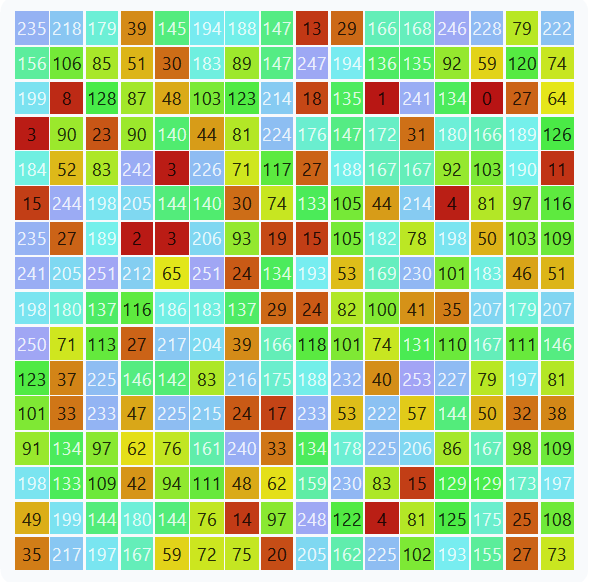
\includegraphics[width=.48\linewidth]{color_representation.png}
\caption{Representation of a lattice through colors} \label{fig1}
\end{figure}

\subsubsection{Matrix Visualization}

\subsection{Visualization Method Effectiveness}
Visualizations as previously defined have been used in education since. Nowadays, it is not hard to find visualization tools for subjects relating to computer science, specifically to cryptography.

\section{Visualization Tool Design}
The developed visualization tool is a web application that provides visualizations for ML-KEM, ML-DSA, LLL, and BKZ. (elaborate later)

\subsection{Architecture}
The visualization tool is built using Next.js, a React-based framework, for the frontend, and primarily Typescript for the backend processes. The ML-KEM and ML-DSA algorithms are implemented using an existing Javascript library and imported as needed. (insert diagram later + be more thorough)

\subsection{ML-KEM}
The implementation of ML-KEM is a modified version of the algorithm privided in the pqc library\cite{pqc-vizz}. 
\subsection{ML-DSA}
This part is for explaning how ML-DSA is implemented/how the code works
\section{Results?}


\section{Conclusion}
\begin{theorem}
This is a sample theorem. The run-in heading is set in bold, while
the following text appears in italics. Definitions, lemmas,
propositions, and corollaries are styled the same way.
\end{theorem}

%
% ---- Bibliography ----
%
% BibTeX users should specify bibliography style 'splncs04'.
% References will then be sorted and formatted in the correct style.
%
\bibliographystyle{acm}
\bibliography{thebibliography}
%
\begin{thebibliography}{8}
\bibitem{fips_203}
National Institute of Standards and Technology. (2024). Module-Lattice-Based Key-Encapsulation Mechanism Standard. \textit{Federal Information Processing Standards Publication}. \doi{10.6028/NIST.FIPS.203}

\bibitem{fips_204}
National Institute of Standards and Technology. (2024). Module-Lattice-Based Digital Signature Standard. \textit{Federal Information Processing Standards Publication}. \doi{10.6028/NIST.FIPS.204}

\bibitem{shor}
Shor, P.W. (1994). Algorithms for quantum computation: discrete logarithms and factoring. \textit{Proceeding 35th Annual Symposium on Foundations of Computer Science}. \doi{10.1109/SFCS.1994.365700}

\bibitem{kyber}
Avanzi et al. (2021). CRYSTALS-Kyber. https://pq-crystals.org/kyber/data/kyber-specification-round3-20210804.pdf

\bibitem{pqc-vizz}
Kalava et al. (2025). Post-Quantum Security for Web Applications. https://pqc.nithinram.com/Post-Quantum%20Security%20for%20Web%20Applications.pdf

\bibitem{mwle}
Langlois, A. \& Stehle, D. (2012). Worst-Case to Average-Case Reductions for Module Lattices. https://eprint.iacr.org/2012/090

\bibitem{metastudy}
Hundhausen, C. D., Douglas, S. A., \& Stasko, J. T. (2002). A Meta-Study of Algorithm Visualization Effectiveness. \textit{Journal of Visual Languages \& Computing}, 13(3), 259–290. \doi{10.1006/jvlc.2002.0237}

\bibitem{daaal}
Stasko, J., Badre, A., \& Lewis, C. (1993). Do Algorithm Animations Assist Learning? An Empirical Study and Analysis. \textit{Proceedings of the SIGCHI Conference on Human Factors in Computing Systems  - CHI ’93}, 61–66. \doi{10.1145/169059.169078}

\bibitem{eaasailca}
Byrne, M. D., Catrambone, R., \& Stasko, J. T. (1999). Evaluating animations as student aids in learning computer algorithms. \textit{Computers \& Education}, 33(4), 253–278. \doi{10.1016/s0360-1315(99)00023-8}

\bibitem{quantumcomputing1}
Benioff, Paul. (1980). The computer as a physical system: A microscopic quantum mechanical Hamiltonian model of computers as represented by Turing machines. \textit{Journal of Statistical Physics}, 22(5), 563–591. \doi{10.1007/bf01011339}

\bibitem{quantumcomputing2}
Benioff, Paul. (1982). Quantum mechanical hamiltonian models of turing machines. \textit{Journal of Statistical Physics}, 29(3), 515–546. \doi{10.1007/BF01342185}

\bibitem{feynman}
Feynman, Richard. (1982). Simulating Physics with Computers. \textit{International Journal of Theoretical Physics}, 21(6/7), 467–488. \doi{10.1007/BF02650179}

\bibitem{}
Bennett, C. H. \& Brassard, G. (2014). Quantum cryptography: Public key distribution and coin tossing. \textit{Theoretical Computer Science. Theoretical Aspects of Quantum Cryptography – celebrating 30 years of BB84}, 560(1), 7–11. \doi{10.1016/j.tcs.2014.05.025}

\bibitem{}
Brassard, G. (2005). Brief history of quantum cryptography: A personal perspective. \doi{10.1109/ITWTPI.2005.1543949}


\end{thebibliography}
\end{document}
